\documentclass[a4paper]{report}

% Packages
\usepackage{enumitem}
\usepackage{graphicx}
\usepackage{array}
\usepackage{float}
\usepackage{url}
\usepackage[maxbibnames=5,style=numeric,backend=bibtex,sorting=nty,firstinits=true]{biblatex} \bibliography{ref}
\usepackage[noabbrev,capitalise]{cleveref} 
\usepackage{tabularx}
\usepackage{tabu}
\usepackage{longtable}
\usepackage[british]{babel}
\usepackage[font=footnotesize]{caption}
\usepackage{csquotes}
\usepackage{color}

% Settings
% Margins in lists
\setlist[itemize]{noitemsep}
% Margins in tables
\renewcommand{\arraystretch}{1.3}

% Text replacement commands
\newcommand{\ie}{i.e.,}
\newcommand{\eg}{e.g.,}
\newcommand{\IVF}{IVF}
\newcommand{\PRN}{PRN}
\newcommand{\AMC}{AMC}
\newcommand{\project}{IVF-PRN project}
\newcommand{\ivfsystem}{IVF-PRN system}
\newcommand{\escience}{e-Science}

% Block comment command
%\long\def\/*#1*/{}

% Commenting commands
\newcommand{\sil}[1]{\textcolor{red}{\textbf{*Silvia: }\textit{#1}}}
\newcommand{\allard}[1]{\textcolor{red}{\textbf{*Allard: }\textit{#1}}}
\newcommand{\note}[1]{\textcolor{cyan}{\textit{#1}}}

% Flag for document style switch, set to true or false
\newif\ifstructure

%\structuretrue
\structurefalse

\title{Thesis}

\author{
	Allard J. van Altena\\
	University of Amsterdam\\
	Email: a.j.vanaltena@amc.uva.nl
}

\begin{document}

	%\maketitle
	
	%\tableofcontents
	
	\chapter{Introduction}
	\label{introduction}
	
	\ifstructure
		What is the problem

What is the IT problem

What is the clinical background

Can it be extrapolated to other backgrounds (should not be here, but keeping it as point of interest)

What is big data and how  does it link into this problem (can be one full section instead of paragraph)

What do we propose to do to help with the problem

How will the proposed system help with the problem

Link back to big data problems

What are the research questions
	\else
		
%TODO: Check if terminology is explained, IVF, PRN, clinical audit registration, \ivfsystem{}, \project.

Right now success percentages of IVF clinics are being published as this is required by law, however they complain that this is unfair as the patient mix between clinics is ‘unfair’. 
IVF clinics want to cooperate in the research of the AMC because they think it is important but they are scared that outcomes will be published in a way that will reflect directly on individual clinics.
In the longer run the AMC wants to profile itself as a knowledge hub for the clinics. The clinics can come to the AMC with questions about the data that is in the project and the AMC can provide answers, advice, or a (sub)set of the data.
As ultimate goal to give the project value the plan is to provide a quality assurance service for the government and the clinics themselves.
This idea can be explored with the NICE registration, they do something like this for Intensive Care units in the Netherlands. 
A doctor can find his or her hospital in the database and compare it versus a subset of ten comparable hospitals or versus the all the hospitals in the Netherlands. 
This registration is used to find points where improvement can be made or as a quality assurance.
Because the clinics are scared that the data will be used against them it will be important to show value of the system and make data collection and security transparent.
Most of the clinics are using the same database software called LSFD. 
To extract data it is no problem to create a query on the system but knowledge of the system is needed before we can do this, thats why we need an appointment with someone who has this knowledge. 
I will try to make an appointment together with Martina (PhD) to visit someone involved in the development of this software to find out how we can extract data from it. 
At this appointment I will try to find out if a direct extraction from a automated system without involvement of personnel is possible.
Anita found a problem in the clinical questions, mine and Alexanders were basically the same. 
I’ve changed my question and will leave it open for change during the project as Martina will also pick up one of the questions. 
The possible subjects are: IVF ICSI, fresh/cryo, type of medium, oxygen tension (?, zuurstofspanning in Dutch).
	\fi

	\chapter{Security}
	\label{security}
	
	\ifstructure
		\newline

8 pages

\section{Security}
\subsection{Literature Review}
\paragraph{Medical big data ethics and security}
Might move big data to another section (introduction?).

\paragraph{The `how?' and `why?' of security}

Why is security needed, background information.	
Integrate literature on security and introduce some concepts of security that were described.

\paragraph{The legal side of security}
Integrate Dutch law into the security, there are some requirements that need to be met for a system to be legal.

\subsection{Interviews}
\paragraph{Set-up}
Description of the interviews taken and what information was gathered there.

\subsection{Interview}

\subsection{Technical \& Procedural Cornerstones of Security}
Table of items that were distilled from literature and interviews.

\subsection{Analysis}
Analysis, how do the security items apply to the system.
	\else
		\section{Literature Review}
\label{security-literature}

\paragraph{Medical big data ethics and security}
\label{security-ethics}

We could start with answering the question 'how do I secure data?', but before doing this it is important to describe what the incentives are for using the data.
We do this to give context to the found security issues and proposed solutions for them.

In 2013 \cite{s20Groves2013} estimated big data strategies could increase profits in US healthcare by \$100 billion \cite{s13Patil2014}.
However to make this possible healthcare management have to change their business model.
Old models worked with increasing or decreasing the amount of patients while the outcome (quality) remained the same, \cite{s13Patil2014} calls this a volume-based business model.
To make the increase in profits possible new models revolving around cost versus quality are used, called a value-based business model.
Much more is written about the pros and cons of this type of healthcare management by gurus like M.E. Porter, but this is outside the scope of this paper.
In order to measure the quality indicators in the new strategies big data can be applied \cite{s6West2009}, through data mining patient outcomes can be linked directly with treatment, environmental factors, or any other data sets.
Choosing the right treatment for any given new patient will then be a matter of checking the charts.
This way of delivering healthcare is also supported by the European Union which describes it as ``Free Movement'' and obtaining quality and efficient healthcare \cite{s8FernandezAleman2013}.
The new set-up closely fits to a standard research set-up.
Data in patient records is mainly used to provide information for caretakers but can be very valuable in research\cite{s15Fenz2014}.
The extraction of data is not very straightforward and should be done with caution as there are security and privacy pitfalls.

According to Fenz \cite{s15Fenz2014} patients will not withhold their data for research purposes.
However, there are concerns that data can be accessed by persons with unwanted intentions: marketing, insurance, or data loss through breaches.
It is positive that big data can help the improvement of healthcare \emph{and} patients are willing to give their data towards this end.
However, data breaches should never be dismissed, which makes the application of big data an ethical question: Does the benefit of the big data overcome the possible negative effects of a data breach.

\cite{s7Kluge2007} took ``What should be the driver of its development and implementation?'' as the context and split the ethical issue into four different questions, respectively: Should it be the technology itself? Should it be the interests of service providers? Should it be the interests of governments? Should it be the interests of patients?
Each of these questions should be dealt with in the \project{}:

\begin{itemize}
	\item \textbf{Should it be the technology itself? -} Because this system is developed in the interest of a research the technology has a stake in the driver of development.
	However, it should not become the main driver as that would destroy the initial idea of improving quality and efficiency of care.
	\item \textbf{Should it be the interests of service providers? -} Service providers are accounted for as they will finally be able to get a impartial comparison between each other.
	If the feedback to providers is delivered in the right manner this should provide both the incentive \emph{and} the knowledge to improve efficiency.
	\item \textbf{Should it be the interests of governments? -} Because the \project{} is the first to look into the coupling of outcome data with \IVF{} data the holy grail to be reached is that the system provides the same services as registries like the NICE\footnote{https://www.stichting-nice.nl/} or  BHN\footnote{https://www.bhn-registratie.nl/}.
	These services include reporting back to the government, these reports make it possible to make informed guidance decision.
	\item \textbf{Should it be the interests of patients? -} The main outcome of the \project{} is to provide insight in outcomes on different \IVF{} treatments.
	A study with these outcome measurements and this size has not been performed yet in the Netherlands.
	The outcomes of a study like this will determine what the best treatment is, and to conduct a study like this the \ivfsystem{} will support the researchers.
\end{itemize}

There are some ethical issues that also involve legal issues like the USA Patriot Act, this will be touched upon in the paragraph \emph{the legal side of security}.

\paragraph{The 'how?' and 'why?' of security}
\label{security-how-why}

When speaking of security in the medical sector the topic can be discerned into several fields according to Perakslis \cite{s2Perakslis2014}: data loss, monetary theft, attacks on medical devices, and attack on infrastructure.
Because the main scope of this study is clinical research data, and thus protecting patient privacy, we will focus on data loss (\ie{} data security).
The use of technology is emerging in the healthcare sector, this results in systems with increased complexity, diversity, and timeliness \cite{s13Patil2014}.
As these systems grow it becomes harder and harder to prevent data breaches.
Furthermore, the healthcare domain is being heavily targeted, 94\% of all institutions have had to deal with attacks on their systems \cite{s2Perakslis2014}.
It is reported that there is more risk of insider attackers, both intentional and unintentional (\eg{} regular employees not following policies) \cite{s1Zamosky2014}.
Only 7\% of all breaches are caused by hacking, mundane errors like stolen laptops are more common \cite{s1Zamosky2014}.
The most common breaches are unauthorised access of data (63 \%) and exposure of sensitive data (57\%) \cite{s18Kum2014}.

About 48\% of data breaches can be traced back to theft with identity theft being the most important one \cite{s1Zamosky2014}.
An obvious factor in this is that the value of stolen data is much higher than in other domains.
The per-record value is directly bound to the amount of data in the record, medical records contain more information than for example financial records which makes them more valuable \cite{s1Zamosky2014}.
It has been estimated that the cost per-record is approximately \$233 in healthcare, while the mean of all industries was \$136 \cite{s2Perakslis2014}.
Next to financial gain there are also hackers that seek to crack a system to deface an institution or to prove that not enough security was in place to start with.
The question we seek to answer in the section is what regulations and conventions should be taken into account when storing and processing data specific to our \ivfsystem{}?

There are three goals that work towards achieving a secure system: confidentiality, integrity, and availability \cite{s8FernandezAleman2013}.
Confidentiality refers to the rights of the patient concerning their personal medical data, what these are will be described in the next paragraph.
Integrity refers to completeness and correctness of data, and availability is reached when the correct person can access the correct data at the correct time (\eg{} clinician accesses a patients' file during a consult).

As the \ivfsystem{} does not influence patient care directly integrity and availability are of less importance.
The importance of confidentiality is also reflected in the following quote: "They wanted to help achieve these benefits but also wanted to be sure that patients' rights were protected and that clinicians were not in danger of breaking patient confidentiality and the law" taken from Sanderson \cite{s5Sanderson2004}.
Clinicians see the benefits of systems supporting them in their daily work but they need to be sure that they are safe to work with.
Furthermore, \cite{s4Layman2008} states that the chance of achieving success with a health informatics system decreases when confidentiality is violated.
The next paragraph will go into the laws and regulations which help to achieve the security goals.

\paragraph{The legal side of security}
\label{security-legal}

While systems grow and hackers become more eager in hacking them lawmakers have put regulations and laws in place to protect patients.
The IT is agile while regulations (unfortunately) are mostly slow-moving \cite{s20Groves2013}, this makes it difficult to cover every important point of privacy in regulations.
Therefore, it should be noted that compliance to these regulations will not necessarily be sufficient for good security \cite{s20Groves2013}.
This paragraph will describe what regulations are in place, only major points will be given as an in-depth explanation is outside of the scope of this research.

Healthcare institutions have to comply to regulations like the EU or US privacy directive.
If they do not there are acts in place that allow government bodies to impose fines.
These fines are becoming larger as the importance of protection of privacy is growing \cite{s1Zamosky2014}.
Respectively the EU directive is 95/46/EG and the US directive Health Insurance Portability and Accountability Act (HIPAA).
For Dutch institutions only the EU directives apply but the HIPAA also gives a good overview of what topics are important for privacy protection.
Also, the EU and US directives are comparable to each other which makes it easier to find technical privacy solutions (described in \ref{security-summarisation}).
The EU directives are implemented in the Netherlands and supplemented with other acts, these are listed with the important parts as described by Mouw \cite{s19Mouw2012}.

\begin{itemize}
	\item Data Protection Act (WBP) - Wet Bescherming Persoonsgegevens (WBP), this is the implementation of the EU directive.
	A government body is granted permission to enforce this implementation and impose fines.
	This act describes when and how data can be collected from a person.
	The most important point to take from this regulation is that specific consent is required before data can be collected and processed.
	\item Medical Contract Bill (WGBO) - Wet Geneeskundige Behandelingsovereenkomst (WGBO), this is an overall act for medical treatment but it also describes regulations for record keeping.
	The most important regulation here is article 458: statistical or medical research in the benefit of public health are exempted from consent regulations if the consent required is impossible or unreasonable to obtain.
	\item Medical Research Involving Human Subjects Act (WMO) - Wet Medisch-wetenschappelijk Onderzoek met mensen (WMO), this regulation is an extension to the WGBO and requires an ethical committees approval for each new medical research.
	\item Code of Conduct for Medical Research (FMWV) - This code of conduct provides concrete examples and implementations of each law mentioned above.
	This makes it easier for medical researchers to comply to each of these laws.
	The code requires that personal data is only accessible by the researcher or those directly under their authority.
\end{itemize}

Furthermore, there is one US act that is also of interest for institutions world-wide, namely the US-based Patriot Act.
The Patriot Act is an odd act in this section, it is mentioned because it endangers patient privacy from countries outside of the US.
If a third party is used for data storage, and this third party has its head quarter in the US, government bodies of the US can request (and will most likely receive) insight into this data \cite{s7Kluge2007}.
This issue should be considered while developing a system that handles patient data.

%Need to find those standards and examine them
Next to legal items there are also some standards that can be applied, these are ISO EN13606 and the NEN7510.
For example the EN13606 defines confidentiality as 'process that ensures that information is accassible only to those authorised to have access to it' \cite{s8FernandezAleman2013}.

Summarising, the laws state that in principle patient data cannot be stored or processed.
However if there is a public interest, like public health, some data may be used \cite{s19Mouw2012}.
In any case personal (\ie{} identifying) data should always be separated from the rest of the data.
Types of data such as religion, race, and sexual preference are excluded and may only be stored when the law explicitly permits it \cite{s19Mouw2012}.
When there is a public interest data usage is possible when each included patient gives his/her explicit consent.
When consent is asked a clear description of the goals for the data should be given.
Also, the patient remains the right to inspection and removal of his/her data from the dataset.
An exception to the consent rule is made when requests are impossible or unreasonable to make.
Furthermore, the law states that medical research can only be done when : "(I) new scientific insights in medicine are expected, (II) those insights cannot be gained in another, less risky way, and (III) the risks for and interest of the participants is well balanced against the importance of the research." \cite{s19Mouw2012}.

The FMWV code of conduct describes the following points which are applicable to this research:

\begin{itemize}
	\item For personal data, the reason of use should be described.
	\item The persons authorised to view personal data should be listed.
	\item Provisions taken to protect the data should be listed.
\end{itemize}

Lastly, an ethical committee is needed to check the usage of data versus the goal of the research.
If it is found that the means do not serve the goal the research cannot continue.

The intent of these laws can be described in a great quote from Aleman \cite{s8FernandezAleman2013}: "the claim of individuals, groups, or institutions to determine for themselves when, how, and to what extent information about them is communicated to others".
		\subsection{Interviews}
\label{security-interviews}

Next to the literature search interviews were held to provide examples for the laws and regulations which are quite abstract.

\paragraph{Set-up} 
\label{security-set-up}

Semi-structured interviews were performed with system security and medical registration system experts.
This interview technique leaves the interviewees free to roam to other subjects which might prove useful in the design of the \ivfsystem{}.
During the interviews firstly the vision of the \ivfsystem{} was explained in a few sentences.
After this the following questions were used to give structure to the interview, the term \emph{personal data} refers to identifying data.

\begin{itemize}
	\item What can we do to make sure we are not processing personal data?
	\item What are the criteria for something to be personal data or not?
	\item If personal data is being processed how can we comply to the extensive rules?
	\item How are things handled in existing registries?
	\item Are these registries also used for research?
	\item Aggregate data in public databases can become individually identifiable when the databases are integrated or the data are cross referenced, how do you account for this?
	\item Facing problems with getting go-ahead from ethical commissions for gathering data, how can a system like the \ivfsystem{} support in getting consent?
\end{itemize}

\subsubsection{First interview}
\label{security-first-interview}

This interview was with an expert on the topic of an intensive care registry in the Netherlands (NICE).
The NICE contains sensitive data where normally consent is required. 
However, patients at the IC are generally non responsive which means that getting consent is an unreasonable requirement and can be disregarded.

Considering consent there is a difference between historical data and \emph{active} data.
When using historical data it is difficult to get consent from each patient providing more room in the interpretation of the law.
For active data it is fairly easy to provide patients with a consent form when they visit the clinic thereby binding the researchers to acquire consent.

It is difficult to avoid processing personal data, \ie{} what is defined by `personal data' is open to interpretation.
Therefore, each of the used data items that might be debatable should be supported by a purpose/goal. % What sounds better?
Goals may vary but most of the time they describe why a certain data item is inevitable to use when doing research with the dataset.
A good guideline when creating a dataset is to take the minimum amount of data items while still being able to fulfil the research goal.
Some categories of data weigh more in a decision than others, \emph{sensitive} items (\eg{} race, sexual preference) are more likely to be turned down.
Once more, for ethical commissions the purpose of data collection and processing is leading in a decision, a well described protocol and application of standards (\eg{} NEN7510) are other points of interest.

It is impossible to guarantee that privacy is always kept.
This is due to factors like public datasets, news, and all other sorts of information sources.
When aggregating these datasets into one big dataset it becomes easier to discern individuals. 
For example, the Dutch queen is hospitalised and this information is published in a newspaper, from other sources (wikipedia, etc.) age and gender can be gathered.
With this information, even though the NICE is considered anonymous, the subset of possible patients can be reduced until in the end only one patient remains.
In order to avoid these kinds of data breaches some precautions can be taken but these will never be completely safe as there is a human factor.
Precautions that should be considered are: take notice of modern technical security techniques and implement those, keep external access to data either off-line or require to go through an internal administrator (\eg{} data extraction requests), aggregate data that is communicated to external sources which removes the likelihood of an individual being identified, when direct access to data is needed (\eg{} administrators, data mining research) use confidentiality documents, direct access to data is bound by location (\eg{} on one specific computer or inside a network).

As a side note, while talking about confidence people have with a system two topics came up.
The NICE makes it possible for ICs to benchmark themselves against data of other clinics.
However, all clinics remain anonymous which avoids discussion about accountability, \eg{} it is highly likely that the worst ranked IC receives less income once it is identified (less patients willing to go there, insurance is unwilling to pay).
The other topic is objectiveness of outcome measures.
Quality indicators that are presented by the system should never be directly influenced by humans, this introduces data playing problems where clinics artificially try to improve their scores by giving patients better outcomes than they actually have.
		\section{Technical \& Procedural Cornerstones of Security}
\label{security-summarisation}

The outcomes of the interviews were combined with the literature study to compile a practical list with security issues and solutions that are relevant in this project.
The list is described in table \ref{tab:security-list}, ordered by type and paper.

Furthermore, two checklists were found in the literature.
These lists give a number of points which a system should comply to in order to cover all identified security areas.
The first list describes items used to test the safety of an implementation of a patient-centred eHealth solution \cite{s17Dehling2014}.
This check list (Checklist A) can be found in appendix \ref{security-checklists-a}.

The second list describes questions used to test EHR systems on security and privacy \cite{s8FernandezAleman2013}.
This check list (Checklist B) can be found in appendix \ref{security-checklists-b}.

% Security table with a list of all found problems and solutions in literature and interviews
\begin{center}
	\renewcommand{\arraystretch}{1.3}
	\begin{longtabu}{c X}
		\caption{List of identified risks and solutions, sorted according to type} \label{tab:security-list} \\
		\hline
			\multicolumn{1}{c}{\textbf{Ref.*}}	&	\textbf{Description} \\
		\hline
			\multicolumn{2}{c}{Procedural problems \& risks} \\
		\hline
			\cite{s4Layman2008}, \ref{security-first-interview}	&	Data aggregation and cross referencing makes the identification of individuals possible. \\
			\cite{s18Kum2014}	&	Applying secondary data analysis makes it difficult to cover purpose in the consent process. \\
			\cite{s18Kum2014}	&	Data linkage without identifying data is impossible, data linkage with identifying data is unsafe. \\
			\cite{s18Kum2014}	&	In data linkage privacy has to be temporarily breached in order to identify matching entities in two datasets. \\
			\cite{s18Kum2014}	&	Finding the right amount of identifying data for linkage is a difficult task. \\
			\ref{security-first-interview}	&	Determining identifying data is open to interpretation. \\
		\\ %whitespace
			\multicolumn{2}{c}{Procedural solutions} \\
		\hline
			\cite{s3Herveg2014}	&	Personal data can only be used for the purposes described when the consent was given by the subject. \\
			\cite{s3Herveg2014, s6West2009, s18Kum2014}, \ref{security-first-interview}	&	Data being used should be in a minimum dataset, no superfluous data should be present. \\
			\cite{s3Herveg2014, s15Fenz2014}	&	After the purpose described in the consent has been reached identifying data should be removed from the dataset. \\
			\cite{s3Herveg2014}	&	The purpose of data usage should be: ``specified, explicit, and legitimate''. \\
			\cite{s8FernandezAleman2013}	&	At any point in time and audit of data should be kept, \ie{} provenance of data. \\
			\cite{s8FernandezAleman2013}	&	Accountability is a central part of security. \\
			\cite{s15Fenz2014, s13Patil2014}	&	Apply anonymisation and pseudonymisation to protect identifiable data or to make it impossible to use this data to identify individuals while still being able to use this data for analytical purposes. \\
			\ref{security-first-interview}	&	For each debatable data item describe the purpose it fulfils. \\
		\\ %whitespace
			\multicolumn{2}{c}{Technical solutions} \\
		\hline
			\cite{s6West2009}	&	Use hashes of identifying data to refer to individuals, which is usable for analytical purposes but not for identifying individuals in the real world. \\
			\cite{s6West2009}	&	Store a specified data structure on a secure server. \\
			\cite{s11Rauscher2014}	&	Use ``portholes'' to view data, \ie{} aggregate data for the user to view but do no disclose the dataset. \\
			\cite{s11Rauscher2014}	&	Declassify data when output is requested by the user, hereby removing identifiable data. \\
			\cite{s16Ma2013}	&	Separate identifying data from dataset, in this paper applied to optimise search. Non-identifying data is available for fast search, after making a selection identifying data is appended before outputting. \\
			\cite{s18Kum2014}	&	Using hashes together with (for example) Bloom filters provide a solution to using identifiable data in data linkage. \\
			\ref{security-first-interview}	&	Take note of standard security measures of the present and implement those. \\
	\end{longtabu}
	\par \bigskip
	*: Reference, either refers to a citation (with brackets []) or an interview (paragraph numbering \eg{} 1.2.1)
\end{center}
%PROCEDURAL
%solution
%TODO: 6 Limited dataset under 45 CFR §164.514(e): 'Under certain circumstances, a covered entity may use and disclose protected health information (PHI) in a limited dataset for research, public health, and health care operations purposes. The privacy regulation identifies a list of identifiers that must be removed from data in order for it to be considered a “limited dataset”. Once removed, the information is not deidentified – it is still PHI governed by the privacy regulation. A data use agreement must be signed by those wishing to use limited datasets.'

\section{Analysis}
\label{security-summarisation-analysis}

Points taken from this security analysis will be described and reviewed in the context of the \ivfsystem{}.

Starting with consent, in the \project{} it can be viewed from multiple perspectives: patient, clinic, and registry.
When a researchers wants to use the dataset available in the \ivfsystem{} they will use data coming from the clinics which in their turn gather data from patients.
This patient data is then linked to the PRN registry data.
Each of the parties involved should to some extent be able to determine if they allow their data to be used.

Patient consent is a difficult problem to tackle in research in general.
When giving consent, patients need to know what they are signing for and handling data outside of the goal which was described is forbidden.
However, when using datasets for which it is unreachable and unreasonable to acquire consent from each patient in them there are exceptions in the Dutch consent regulations.

This exception is what the \ivfsystem{} currently leans on. 
It uses historical data for the years 2000 to 2010 and according to the nationwide IVF report \cite{ivfReportNVOG} there are approximately 4000 pregnancies per year.
Which means that there are about 40.000 patients in the dataset in total.
Given the size and age of the dataset it was deemed unreasonable to require consent.
To determine if consent is not a requirement advice from external parties should be acquired.
In this case these were: the \AMC{} chief privacy officer, medical ethical commissions of data suppliers, and the \PRN{} privacy commission.

Consent from clinics and registries can be compared to patient consent.
They all give permission to use \emph{their} data for a specific cause as described in the consent.
The main difference between these data providers in giving consent is that their considerations are based on different interests.

For example, a patient might be concerned about his/her privacy.
Of course a clinic will also take this into account when a dataset is requested but they also have interests like: what research will be performed with the data.
If this clashes with a research of their own it is less likely the clinic will give consent.
In the \ivfsystem{} these different levels of consent must be taken into account  to be able to perform the function of providing research data.

In order to fulfil regulations and ethical needs a dataset should be minimised so that no superfluous items are left in the dataset.
For each of the data items in the dataset a purpose should be described. 
A proper purpose is leading in ethical discussions about whether to accept a data item in the dataset or not.
Having a well-defined protocol with the \ivfsystem{} can provide more confidence in the system by users, leads to better understanding of the system, and provides evidence that choices about data items were made with certain considerations.

For data linkage some identifying (\ie{} private) data items are needed.
This can be described in the purpose of the data item, but there are also methods for avoiding these data items.
Hashing of data with the application of Bloom filters make it possible to link two datasets without revealing the identifying data.
Data linkage is only mentioned as a future reference for the \ivfsystem{}.
In the first implementation linkage is provided by a third-party.

Anonymisation and pseudonymisation should be used to de-identify individuals.
While identification through data aggregation and cross-referencing is still possible to happen, these steps should make it more difficult.
The \ivfsystem{} will use both techniques to provide privacy, datasets are mostly kept clean by removing all identifying data at the data gathering step.
Whatever identifying data is left (through linkage) will be pseudonymised before it is accepted into the system.

In order to decrease the chances of cross-referencing and data breaches in general, auditing should be applied.
This means keeping logs on who uses what data at what point in time and what that data looked like at that time.
Apart from privacy this also makes it possible to keep people accountable and to provide data management functionality.

Lastly, exploring and using present day standard security measures are a must-have for a good system.
During the software engineering cycle of the \ivfsystem{} searches will be done for the appropriate security measures for each part of the system.
Also the expertise of developers, engineers, and system administrators with multiple years of experience each will be used.
	\fi
	
	\chapter{System Functionality}
	\label{system-functionality}
	
	\ifstructure
		What is data management in the context of the \ivfsystem{}?


Section 1: Brainstorm

How is research normally performed

Workflow description

Initial idea (before brainstorm), where does the system fit into the research workflow

Idea after brainstorm, where does the system fit into the research worflow now?

Differences between ideas

Functions in workflow

What points in the research workflow are supported/improved, differences between before and after brainstorm

Section 2: Rosemary

What is it now > data management system

Functions of Rosemary

Compare to brainstorm functions

Arguments for use of this system: re-use, in-house project, expertise is here, data model fits with minimal change (next chapter).	
	\else
		How is research normally performed

Workflow description

Initial idea (before brainstorm)

Idea after brainstorm

Differences between ideas

Functions in workflow

What points in the research workflow are supported/improved
		What is it, data management system

Functions of Rosemary

Compare to brainstorm functions

Arguments for use of this system: re-use, in-house project, expertise is here, data model fits with minimal change (next chapter).
		What is data management in the context of the \ivfsystem{}?

How does this translate into functionality?

What are the functions?

How was the brainstorm performed and what were the results?

What functionality did we acquire from the brainstorm?
	\fi
	
	\chapter{Data Model}
	\label{datamodel}
	
	\ifstructure
		What context are we talking about in this chapter?

Description of the data, what is being collected now (PRN, clinics)?

How was the data gathered, what were the problems and solutions found here?

Description of the model.

What is data provenance and how is it applied to this model?

How does the data fit inside this model?

What does the model look like on an abstract level (ER?)?
	\else
		This section will give an abstract view and an implementation of the proposed data model for the acquired data.
Firstly the current data used in the \project{} will be described after that the data model used for technical implementation will be described.

\section{Data Description}
\label{datamodel-data-description}

There are two types of data in the \project{}, data coming from the \PRN{} and data coming from the clinics.
The \PRN{} data is fairly structured, there are some changes in the data model over time but overall not much is added or removed.
This differs from the clinics which have a great variance in datasets between each other.
During the \project{} a transition is happening, most (if not all) of the clinics will be adopting a new patient record system (LSFD\footnote{http://stichting-saf.nl/lsfd/}).
This system is developed in coordination with the Dutch foundation for automation of fertility clinics (Dutch: Stichting Automatisering Fertiliteit, SAF\footnote{http://stichting-saf.nl/}).
The SAF embodies the interests of all fertility healthcare providers in the Netherlands and therefore they can make decisions on how to standardise datasets.

In the data model of the \ivfsystem{} it should not be required to have one standardised dataset, at the current time (without the LSFD software) there is no standardised dataset.
The knowledge that at one point in time a standard dataset is available should be taken into account but it is more a data gathering problem.

The data itself is provided in a table-like format with columns and rows.
Data was gathered retrospectively and it is retrieved for the year 1999 up to 2010.
Each of the rows contain a pregnancy and each pregnancy consist of data items that are related to it (columns), \eg{} BMI at the time of impregnation.
Between clinics the provided columns differ from each other, during data gathering there was a protocol describing the requested data items but not all clinics were able to provide these.
Data gathered from the \PRN{} registry is available for each of the rows as the requested data items have not changed over the time period (1999 - 2010).
Most of the identifying data has been stripped and those items that remain are pseudonymised, \eg{} the pseudonym for date of birth is age in years.
After this is done the dataset is received by the \ivfsystem{}.

A first step that needs to be performed is to clean the data and make it usable for computerised processing.
The first data clean up will need to be done by hand, but once an algorithm is defined for a specific dataset further updates can be performed automatically.
Datasets that have been cleaned will be stored in the \ivfsystem{} an abstract model will be described in the following section.

\section{Model Description}
\label{datamodel-model-description}

Initially in the \project it is the case that two datasets (\IVF{} and \PRN{} data) will be linked and stored together.
However, the data model has to be flexible in order to make arrangements for future extensions. 
Both in adding new datasets and in extending existing datasets with more data items.

At the start of the project requirements were identified regarding the data storage. 
Requirements were distilled from literature and interviews from the data security section \ref{security}, and also from interviews performed with stakeholders before starting the project.

\begin{enumerate}[topsep=0pt, itemsep=-1ex]
	\item User and role based access to data;
	\item Keep data provenance;
	\item Datasets can be extended with new data items;
	\item New datasets can be added;
	\item Also keep non-linked data in dataset;
	\item Keep linkage between datasets in a separate entity;
	\item Keep data agreements with the datasets;
	\item Aggregated/statistical data retrieval should be possible.
\end{enumerate}

\paragraph{Compiling the model}
\label{datamodel-compiling}

The first data model for the \ivfsystem{} was developed from these requirements and can be seen in figure \ref{fig:model-drawing}.
Complying to requirement 1, 2, 6, and 7 was straightforward, each of the requirements describes that the data should be stored in a separate entities which is reflected in the model.
Data entities are respectively: {\tt User}, {\tt Provenance}, {\tt Linkage}, and {\tt Data agreements}.

Requirement 3 and 4 both have a need for {\tt Sub collections}, these implement a minimum data item set.
For example, one of the {\tt sub collections} is the \IVF{} dataset, the cross section of available data items for all \IVF{} datasets is the minimum data item set.
This set-up makes it possible to add other (different) datasets but also to extend existing datasets with new data items.

Requirement 5 needs some background information.
In the data linkage process not all rows of data from one dataset will find a corresponding row in the other dataset.
Discarding these rows is not in the interest of the research that can be performed on the whole dataset.
This is where requirement 6 comes in to play, keeping the {\tt Linkage} separately from the {\tt Data} makes it possible to keep all rows (including the non-linked).
Incorporating these possibilities into the data model opens up chances for more functionality in the \ivfsystem{}.

Requirement 8 is based on both security as functional considerations.
The security literature tells us that the raw dataset should be protected against direct access as much as possible.
Therefore, when research is performed on the extracted data certain key data items can be aggregated.
This creates a protection layer against identifying individuals in the extracted data.
For example, (most of the time) it is unnecessary to know the exact age for each of the included patients in a research, in those cases the aggregated mean age of all patients can suffice.

\begin{figure}[!b]
	\centering
	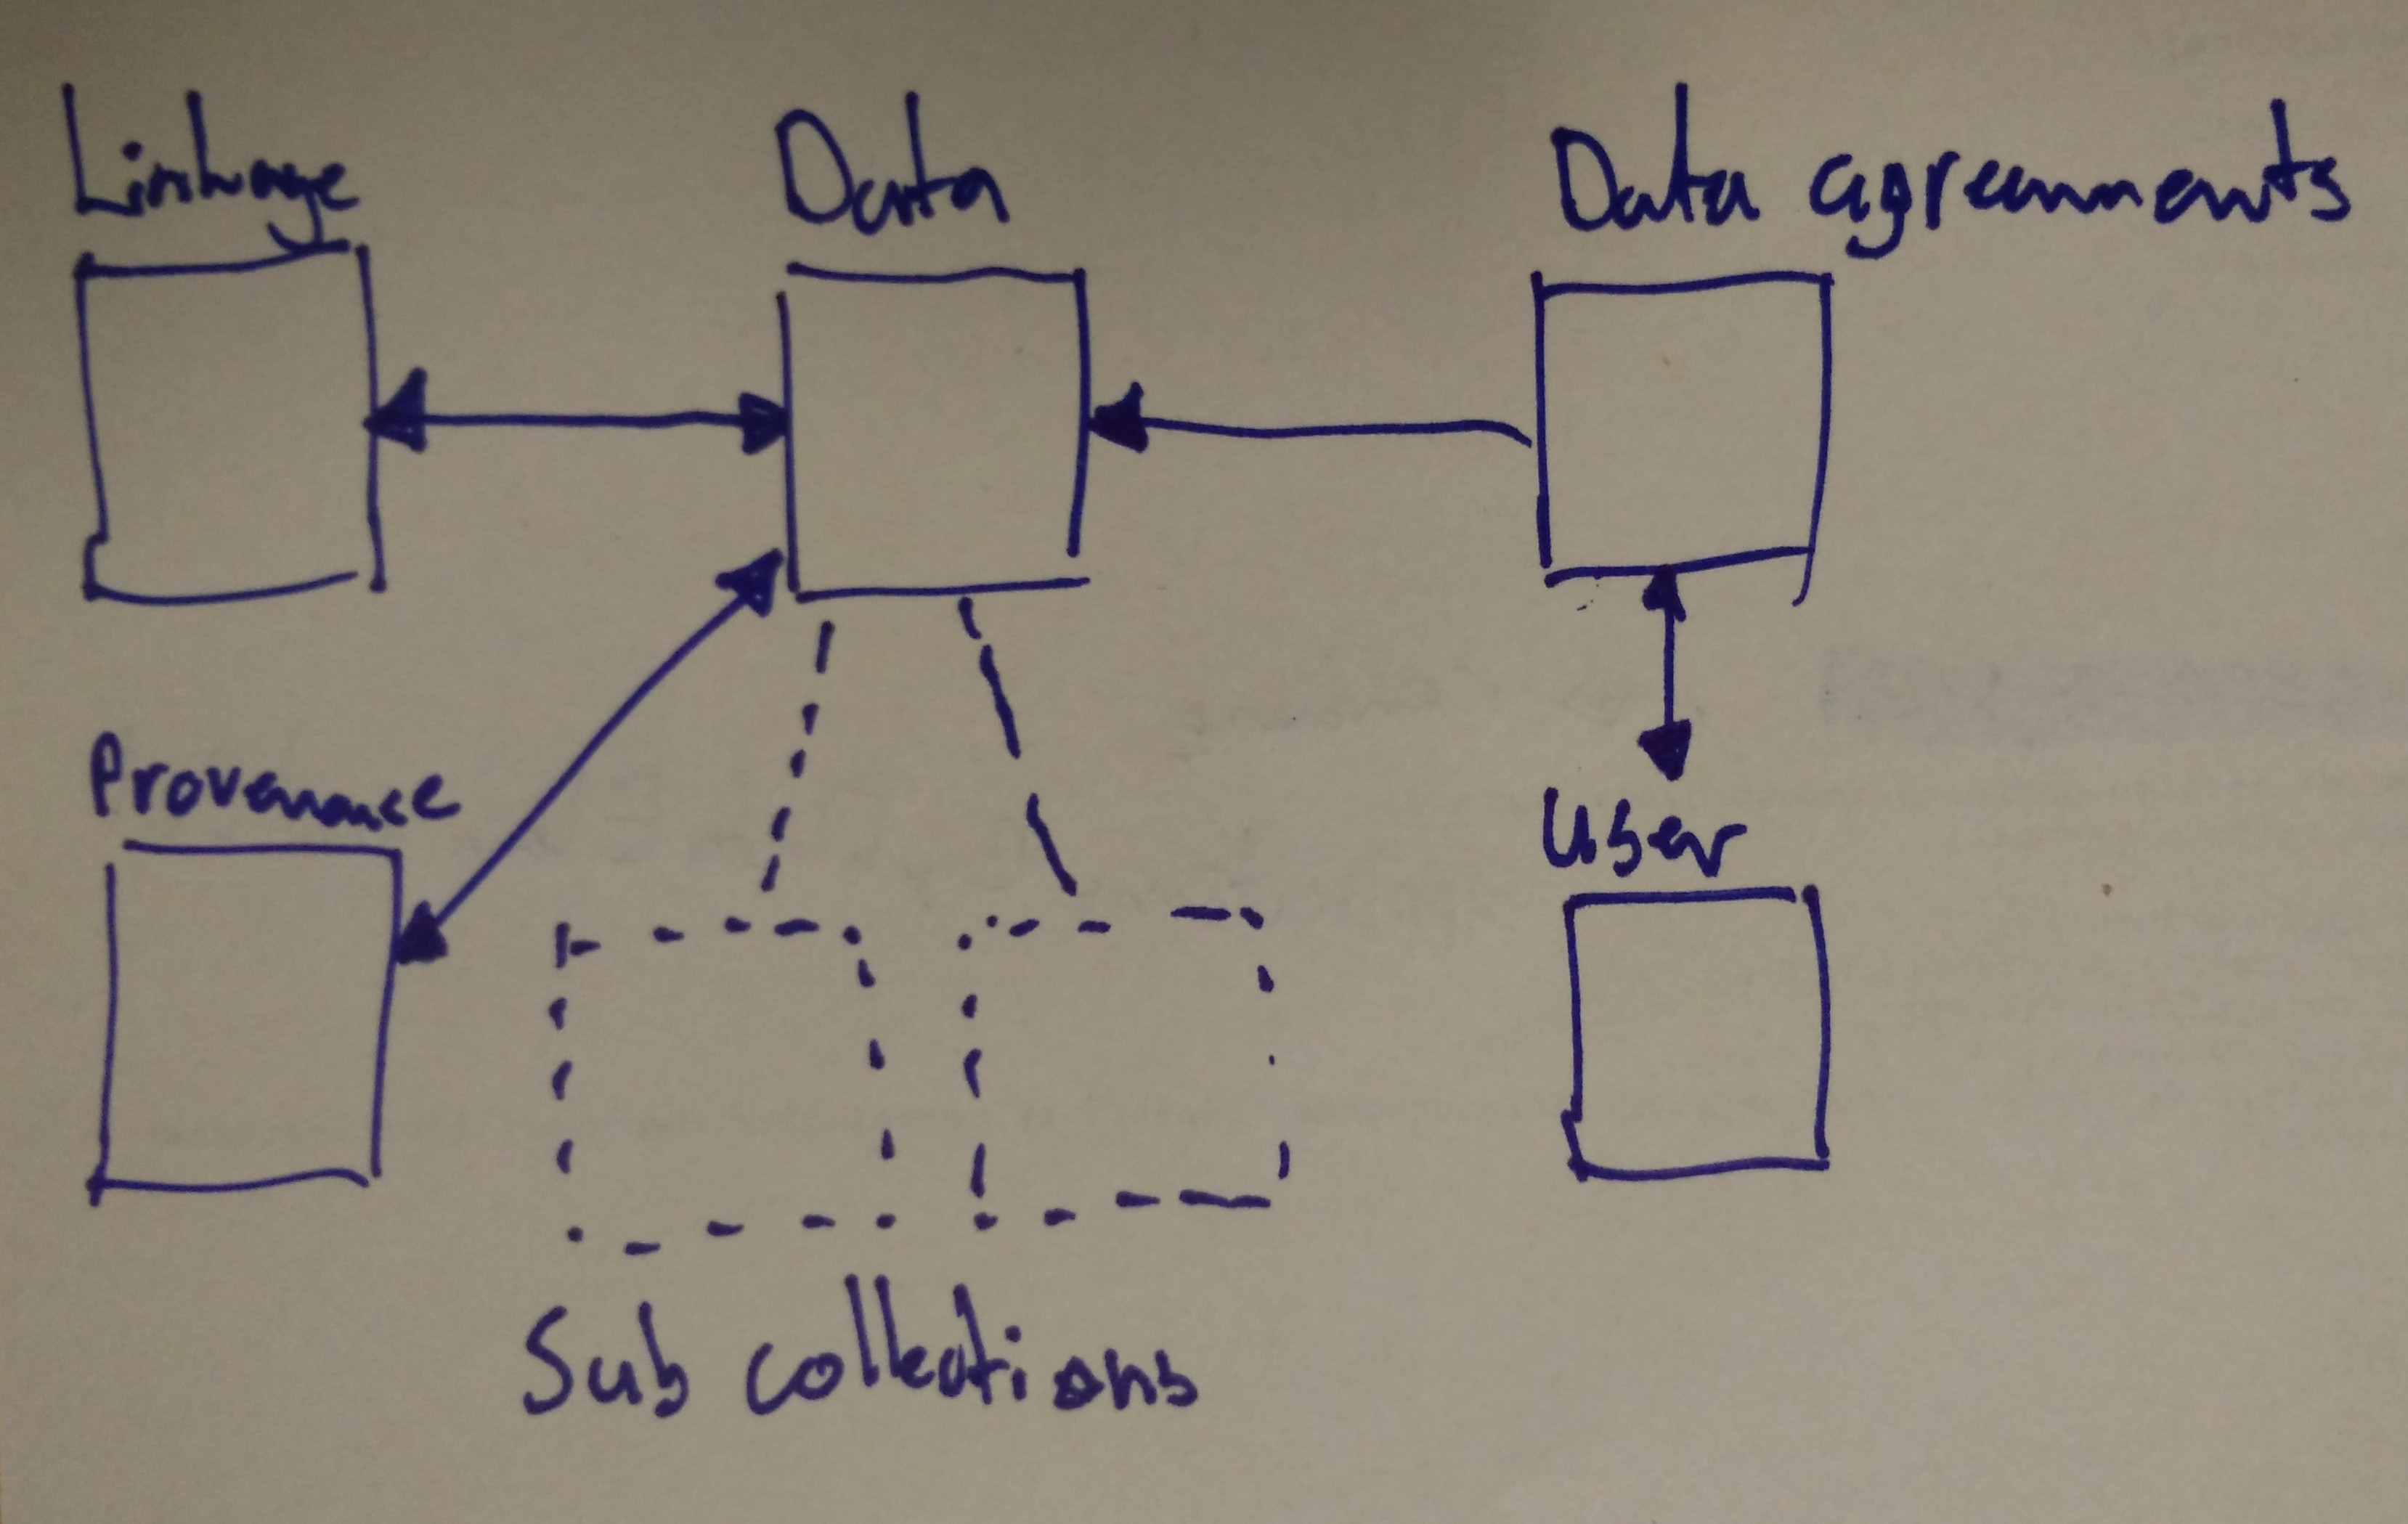
\includegraphics[width=1.0\linewidth]{images/small-structure-v2}
	\caption{Initial drawing of the data model} %TODO: write more caption
	\label{fig:model-drawing}
\end{figure}

\paragraph{Schema(less)}
\label{datamodel-schema}

A choice which is made later in the software engineering part of the project is whether or not to pick a schemaless database.
This point will be elaborated further on in this thesis.
For now it will suffice to say that the identified requirement 3 asks for a schemaless database.

%Part of introduction?
\section{Data Gathering}
\label{datamodel-gathering}

%TODO: compile list of problems

%TODO: what is provenance (literature) and how do I model this?
		% Styling commands for the used terms
\newcommand{\agent}{{\tt agent}}
\newcommand{\entity}{{\tt entity}}
\newcommand{\activity}{{\tt activity}}
\newcommand{\relation}{{\tt relation}}
\newcommand{\relations}{{\tt relations}}
\newcommand{\attributes}{{\tt attributes}}

\section{Data Provenance}
\label{datamodel-provenance}

A topic with growing interest in the \escience{} field is provenance, sometimes also referred to as lineage or pedigree.
It has been borrowed from the world of art where it describes the `life' of an artwork.
Mostly this will be the record of ownership but it can also describe things like restorations.
From provenance data the quality, state, and originality of the work can be discerned.

In \escience{} the same can be applied on a piece of data \cite{dsp4moreau}.
Concerning data, provenance is stored metadata describing the process by which the data got to a certain state from a specific source \cite{dsp4moreau,dsp2buneman}.
To describe the path data has taken W3C has made a standard described in the PROV Model Primer \cite{dsp8gil}.
The gist of provenance is that it is build from a small set of assertions made by the different services that are involved in  the data process \cite{dsp4moreau}.

To actually \emph{use} provenance data a standard for schemas is described which are usable for human consumption, an example is shown in figure \ref{fig:provenance-large-schema}.
Because these schemas can run from the starting point where provenance data was kept (or actually the beginning of all time) user-tailored queries should be applied \cite{dsp4moreau}.
These frame the specific question a user has and only display the applicable part of the schema.

\paragraph{The `why?' of provenance}
\label{provenance-why}

When collecting provenance various metadata has to be captured at different steps in the data process.
This creates a overhead when using a system for a specific task.
Capturing and keeping provenance data is almost never the main functionality of a system.
However, exposing the data may help users (\ie{} researchers).

In \escience{} data is gathered and generated at a fast pace.
Provenance kept of this data can help researchers determine whether data is:

\begin{itemize}
	\item Usable in a certain context, the metadata stored can describe the different uses of a specific data item \cite{dsp1simmhan}, \eg{} types of software that accept a data item as input.
	\item Acceptable, the path a piece of data has taken to get to its current form can tell a researcher if they trust the accuracy and timeliness and accept if for further use \cite{dsp1simmhan,dsp3buneman}.
	\item Protected by intellectual property (IP) or should be credited, as for the acceptability of data the path can also be backtracked to the original creators and/or IP holders \cite{dsp1simmhan}.
\end{itemize}

\paragraph{The `how?' of provenance}
\label{provenance-how}

The provenance building blocks (as described by the W3C \cite{dsp8gil}) are the three core data types (\agent{}, \entity{}, and \activity{}) and a few of the possible \relations{} between them as shown in figure \ref{fig:provenance-overview}.
Furthermore, \attributes{} (not shown) can be assigned to provide more metadata for data types or \relations{}.
Provenance output is also standardised, figure \ref{fig:provenance-overview} shows the display methods for the data types and \relations{}, \attributes{} are displayed with a `document' symbol as shown in figure \ref{fig:provenance-large-schema}.

\begin{figure}[h]
	\centering
	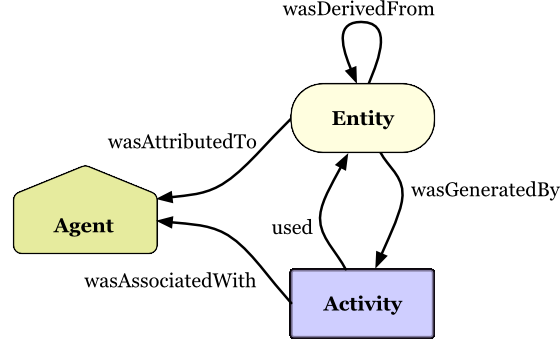
\includegraphics[width=0.5\linewidth]{images/provenance-overview}
	\caption{Example model showing the three core data types (\agent{}, \entity{}, and \activity{}) and a few of all possible \relations{} between them. 
		Taken from PROV Model Primer \cite{dsp8gil}.}
	\label{fig:provenance-overview}
\end{figure}

List of used concepts as described in PROV Model Primer \cite{dsp8gil}:

\begin{itemize}
	\item Entity, physical, digital, conceptual, or another type of `thing'.
	\item Activity, the process of instantiating or the process of changing an entity.
	\item Agent, holds (a part of) the responsibility for activities and entities.
	\item Relation, describes the interaction between two instances of the three core data types.
\end{itemize}

\begin{figure}[!t]
	\centering
	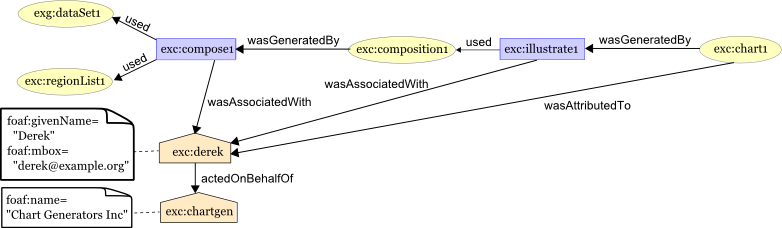
\includegraphics[width=1.0\linewidth]{images/provenance-large-schema}
	\caption{
		Real life example model which implements the model as shown in figure \ref{fig:provenance-overview}.
		This example describes the creation of a chart, the original data used, the intermediate data generated during the process, the used software, who was responsible for the work, and who this person was working for.
		An addition to figure \ref{fig:provenance-overview} is the use of \attributes{}, these are displayed with document icons and provide metadata on the object they are bound to.
		In this case that is the name and email address for one the agents and the company name for the other agent.
		Taken from PROV Model Primer \cite{dsp8gil}.
		}
	\label{fig:provenance-large-schema}
\end{figure}

An provenance example is given in figure \ref{fig:provenance-large-schema}.
Here is shown what the provenance of a certain `chart' is.
The chart (\entity) is shown at the far right side of the figure; it was generated by (\relation) some illustration software (\activity); which in its turn used data from a composition dataset; the data was generated by composing software; two datasets where used in the process, data set 1 and region list.
The agent executing this process is Derek (\agent), he was associated with the composing and illustration software and is attributed to the creation of the resulting chart.
However, Derek is acting on behalf of the company chart gen (\eg{} he is a contractor or employee).
Both agents in this example have \attributes{} assigned to them to further describe them (\eg{} the full name of the company).



HOW
1 Publications are a common form of representing the provenance of experimental data and results.
1 DOIs are used to cite data used in experiments so that the papers can relate the experimental process and analysis to the actual data used an produced.
1 Several applications of provenance: Data quality (based on the provenance meta data a user can check the quality of data), audit trail (who did what with which data), replication recipes (what was done to get a certain data item), attribution (copyright, ownership, citation, liability), informational (data discovery, context for data).

1 If provenance depends on users manually adding annotations instead of automatically collecting it, the burden on the user may prevent complete provenance from being recorded and available in a machine accessible form that has semantic value.
3 why and where provenance, why is data in the output? where does some data in output come from?
4 In order to minimize its effect on application performance, documentation must be structured so it can be constructed and recorded autonomously by services on a piecemeal basis.
4 three types of assertions: relationship (B was retrieved by applying func1 to A), interaction (received A, sent B), service state (it took 3 seconds to send B after receiving A).
	\fi
	
	\chapter{Software Engineering}
	\label{engineering}
	
	\ifstructure
		\begin{itemize}
	\item Small summary of data model and system functions.
	\item Section 1 research:
	\begin{itemize}
		\item What are existing systems for storing medical research data?
		\item Also take Rosemary into account and to other (older) gateways, positive and negative points.
		\item Summary, why did these systems not suffice for our problem.
	\end{itemize}
	\item Section 2 engineering:
	\begin{itemize}
		\item What were the methods applied for the engineering.
		\item Go from methods explaining what the workflow was.
		\item Integrate the brainstorm and updates during iterations of engineering (stakeholders having input on engineering process).
		\item Describe the iterations, what was done, what was achieved, what is left to do.
		\item When code reuse is applied describe it here as well, where it was found and what it brings to this project.
	\end{itemize}
\end{itemize}	
	\else
		Small summary of data model and system functions.

What were the methods applied for the engineering.

Go from methods explaining what the workflow was.

	Integrate the brainstorm and updates during iterations of engineering (stakeholders having input on engineering process).

Describe the iterations, what was done, what was achieved, what is left to do.

	When code reuse is applied describe it here as well, where it was found and what it brings to this project.
	\fi
	
	\clearpage
	
	%\printbibliography
	
	\appendix
	\chapter{Security Checklists}
	\label{security-appendix}
	
	\ifstructure
	\else 
		\section{Checklist A}
\label{security-checklists-a}

This section gives two checklists found in the literature.
These lists give a number of points which a system should comply to in order to be secure in the sense of privacy.
The first list describes items used to test safety of the implementation of a patient-centred eHealth solution in Dehling \cite{s17Dehling2014}:
\begin{itemize}
	\item No unauthorized person must be able to access patients' information;
	\item The real identity of patients must not be revealed;
	\item Access must be limited to necessary information and data segregation must be ensured;
	\item Unnecessary access rights must be revoked;
	\item It cannot be possible to force patients to reveal information they do not want to reveal;
	\item Eavesdropping has to be prevented during transmission and storage;
	\item It must not be possible to reveal relationships between items through observation;
	\item It must be ensured that information content is as intended and not unintentionally changed;
	\item Up-to-date information must be available whenever needed;
	\item Redundancy must be employed to ensure that data can be restored;
	\item It must be possible to store information as long as it is required (even a lifetime or longer);
	\item It must be possible to restore lost information to a specific point in time;
	\item Failure of single nodes must not impede the performance of the whole service;
	\item Systems have to be adaptable to changing performance needs;
	\item There cannot be a significant delay between data entry and dissemination to patients;
	\item Accesses to and uses of information must be attributed to the respective party and it must not be possible to deny such actions afterwards;
	\item Relevant activity (e.g. document accesses) must be logged;
	\item It must be determined who is using the software and verified that they are who they claim to be;
	\item The boundaries of trusted access to the information system must be known and controlled;
	\item Unintended actions and/or activity must be detected;
	\item Unauthorized access must be avoided and access rights must be managed;
	\item Impairment of hardware (theft, natural disasters, ...) has to be prevented;
	\item System vulnerabilities must be detected;
	\item Important information has to be easily accessible;
	\item Patients have to be able to control who can access what information;
	\item Authorization details must be substitutable (loss, technological obsolescence);
	\item User ethics, obligations, and proficiency must be reinforced;
	\item In case of emergency, medical professionals must be able to access required information;
	\item Patients have to agree to uses of their information and patient consent must be managed;
	\item Patients have to be able to retrieve information stored on them.
\end{itemize}

\section{Checklist B}
\label{security-checklists-b}

The second list describes questions used to test EHR systems on security and privacy in Fernández-Alemán \cite{s8FernandezAleman2013}:
\begin{itemize}
	\item What standards and regulations does the system satisfy?
	\item Does the system use pseudo anonymity techniques?
	\item Is the user data encrypted? 
	\item What authentication systems are used? 
	\item Can access policies be overridden in the case of an emergency? 
	\item If the system needs user roles, who defines them? 
	\item Who grants the access to the data? 
	\item What kind of information is exchanged? 
	\item Are there audit logs?
	\item Are the systems' users trained in security and privacy issues? 
\end{itemize}
	\fi

\end{document}
